\chapter{AES Algorithm}

\section{S-Box ($GF(2^8)$)}

Let $m(x):=x^8+x^4+x^3+x+1$.
\begin{align*}
	GF(2^8)&=GF(2)[x]/\langle x^8+x^4+x^3+x+1\rangle \\
	&=GF(2)[x]/\langle m(x)\rangle \\
	&=\set{b_0+b_1x+\cdots+b_6x^6+b_7x^7:b_0,b_1,\cdots, b_6,b_7\in GF(2)}\\
	&=\set{\sum_{i=0}^7b_ix^i:b_i\in\set{0,1}}.
\end{align*}
Let $f(x),g(x)\in GF(2^8)$, say, \[
f(x)=\sum_{i=0}^7a_ix^i+\langle m(x)\rangle,\quad g(x)=\sum_{j=0}^7b_jx^j+\langle m(x)\rangle.
\] Then
\[
f(x)+g(x)=\sum_{i=0}^7(a_i+b_i)x^i+\langle m(x)\rangle=\sum_{i=0}^7(a_i\oplus b_i)x^i+\langle m(x)\rangle.
\] Here, $\oplus:GF(2)\times GF(2)\to GF(2)$. And \begin{align*}
	f(x)\cdot g(x)=m(x)\cdot q(x) + r(x).
\end{align*} Here $\deg r \leq 7$.
\newpage
We define \[
\fullfunction{\texttt{xtime}}{GF(2^8)}{GF(2^8)}{f(x)}{x\cdot f(x)}.
\]
Then \begin{enumerate}
	\item $f(x) = a_0 + a_1x + \cdots + a_6x^6 + a_7x^7$
	\item \begin{align*}
		x\cdot f(x) &= a_0x + a_1x^2 + \cdots + a_6x^7 + a_7x^8 \\
		&= a_0x + a_1x^2 + \cdots + a_6x^7 + a_7(x^4+x^3+x+1)\quad\because x^8\equiv x^4+x^3+x+1\pmod{m(x)} \\
		&=\begin{cases}
			\sum_{i=0}^6a_ix^{i+1} + 0 &:a_7=0\\
			\sum_{i=0}^6a_ix^{i+1} + (x^4+x^3+x+1) &:a_7=1
		\end{cases} \\
		&=\begin{cases}
			(f(x) \ll \texttt{1}) &:a_7=0\\
			(f(x) \ll \texttt{1}) \oplus \texttt{0x1b} &:a_7=1
		\end{cases}
	\end{align*}
\end{enumerate}

\lstinputlisting[style=C]{../doc/codes/GF256_xtime.c}

\begin{align*}
	g(x)\cdot f(x) &= \sum_{i=0}^7g(x)a_ix^i \\
	&= g(x)a_0 + \sum_{i=1}^7g(x)a_ix^i \\
	&= g(x)a_0 + \textcolor{red}{x}\sum_{i=1}^7g(x)a_ix^{i-1} \\
	&= g(x)a_0 + \textcolor{red}{x}\left(g(x)a_1 + \sum_{i=2}^7g(x)a_ix^{i-2}\right) \\
	&= g(x)a_0 + \textcolor{red}{x}\left(g(x)a_1 + \textcolor{red}{x}\left(g(x)a_2 + \sum_{i=3}^7g(x)a_ix^{i-3}\right)\right) \\
	&= \cdots \\
	&= g(x)a_0 + \textcolor{red}{x}(g(x)a_1 + \textcolor{red}{x}(g(x)a_2 + \textcolor{red}{x}(g(x)a_3 + \textcolor{red}{x}(g(x)a_4 + \textcolor{red}{x}(g(x)a_5 + \textcolor{red}{x}(g(x)a_6 + \textcolor{red}{x}(g(x)a_7)))))))
\end{align*}

That is, \begin{align*}
	&x &\cdot& 0 & + & (g(x)\cdot a_7)\\
	&x &\cdot& (g(x)\cdot a_7) & + & (g(x)\cdot a_6)\\
	&x &\cdot& (x\cdot (g(x)\cdot a_7) + (g(x)\cdot a_6)) & + & (g(x)\cdot a_5)\\
\end{align*}\begin{enumerate}[Step 1.]
	\item $x\cdot 0 + g(x)\cdot a_7$
	\item $x\cdot (g(x)\cdot a_7) + (g(x)\cdot a_6)$
	\item $x\cdot (x\cdot (g(x)\cdot a_7) + (g(x)\cdot a_6)) + (g(x)\cdot a_5)$
	\item[] $\cdots$
	\item[Final.] $g\cdot a_0 + x(g\cdot a_1 + \cdots + x(g\cdot a_5 + x(g\cdot a_6 + x(g\cdot a_7))))$
\end{enumerate}

\lstinputlisting[style=C]{../doc/codes/GF256_mul.c}

\lstinputlisting[style=C]{../doc/codes/GF256_MUL.c}

\newpage

\section{MixColumns ($GF(2^8)[x]/\gen{x^4+1}$)}
\[
\fullfunction{\textsf{MixColumns}}{\binaryfield^{128}}{\binaryfield^{128}}{\sum_{i=0}^{127}a_ix^i}{\sum_{j=0}^{127}b_jx^j}
\]

\begin{center}\setstretch{1.5}\begin{tabular}{|c|c|c|c|c|c|c|c|c|c|c|c|c|c|c|c|}\hline
	\cellcolor{red!20} $X_0$ & \cellcolor{red!20}$X_1$ & \cellcolor{red!20}$X_2$ & \cellcolor{red!20}$X_3$ & \cellcolor{green!20} $X_4$ & \cellcolor{green!20}$X_5$ & \cellcolor{green!20}$X_6$ & \cellcolor{green!20} $X_7$ & \cellcolor{blue!20} $X_8$ & \cellcolor{blue!20} $X_9$ & \cellcolor{blue!20} $X_{10}$ & \cellcolor{blue!20} $X_{11}$ & \cellcolor{yellow!20} $X_{12}$ & \cellcolor{yellow!20} $X_{13}$ & \cellcolor{yellow!20} $X_{14}$ & \cellcolor{yellow!20} $X_{15}$ \\ \hline
\end{tabular}\\
$\Downarrow$\\
\begin{tabular}{|c|c|c|c|c|c|c|c|c|c|c|c|c|c|c|c|}\hline
	\cellcolor{red!20} $X_0'$ & \cellcolor{red!20}$X_1'$ & \cellcolor{red!20}$X_2'$ & \cellcolor{red!20}$X_3'$ & \cellcolor{green!20} $X_4'$ & \cellcolor{green!20}$X_5'$ & \cellcolor{green!20}$X_6'$ & \cellcolor{green!20} $X_7'$ & \cellcolor{blue!20} $X_8'$ & \cellcolor{blue!20} $X_9'$ & \cellcolor{blue!20} $X_{10}'$ & \cellcolor{blue!20} $X_{11}'$ & \cellcolor{yellow!20} $X_{12}'$ & \cellcolor{yellow!20} $X_{13}'$ & \cellcolor{yellow!20} $X_{14}'$ & \cellcolor{yellow!20} $X_{15}'$ \\ \hline
\end{tabular}\\
\end{center}

\begin{center}\setstretch{1.5}
	\begin{minipage}{.4\textwidth}\centering
		\begin{tabular}{|c|c|c|c|}
			\hline
			\cellcolor{red!20}$X_0$ & \cellcolor{green!20}$X_4$ & \cellcolor{blue!20}$X_8$ & \cellcolor{yellow!20}$X_{12}$ \\ \hline
			\cellcolor{red!20}$X_1$ & \cellcolor{green!20}$X_5$ & \cellcolor{blue!20}$X_9$ & \cellcolor{yellow!20}$X_{13}$ \\ \hline
			\cellcolor{red!20}$X_2$ & \cellcolor{green!20}$X_6$ & \cellcolor{blue!20}$X_{10}$ & \cellcolor{yellow!20}$X_{14}$ \\ \hline
			\cellcolor{red!20}$X_3$ & \cellcolor{green!20}$X_7$ & \cellcolor{blue!20}$X_{11}$ & \cellcolor{yellow!20}$X_{15}$ \\ \hline
		\end{tabular}
	\end{minipage}$\implies$\begin{minipage}{.4\textwidth}\centering
		\begin{tabular}{|c|c|c|c|}
			\hline
			\cellcolor{red!20}$X_0'$ & \cellcolor{green!20}$X_4'$ & \cellcolor{blue!20}$X_8'$ & \cellcolor{yellow!20}$X_{12}'$ \\ \hline
			\cellcolor{red!20}$X_1'$ & \cellcolor{green!20}$X_5'$ & \cellcolor{blue!20}$X_9'$ & \cellcolor{yellow!20}$X_{13}'$ \\ \hline
			\cellcolor{red!20}$X_2'$ & \cellcolor{green!20}$X_6'$ & \cellcolor{blue!20}$X_{10}'$ & \cellcolor{yellow!20}$X_{14}'$ \\ \hline
			\cellcolor{red!20}$X_3'$ & \cellcolor{green!20}$X_7'$ & \cellcolor{blue!20}$X_{11}'$ & \cellcolor{yellow!20}$X_{15}'$ \\ \hline
		\end{tabular}
	\end{minipage}
\end{center}

\newpage
\noindent Consider
\[
GF(2^8)[x]/\gen{x^4+1}=\set{a_0+a_1x+a_2x^3+a_3x^3: a_i\in GF(2^8)}.
\] Note that $x^5=(x^4+1)x+x\equiv x\pmod{\gen{x^4+1}}$.
We choose \[
a(x)=(\texttt{0x03})\cdot x^3 + (\texttt{0x01})\cdot x^2 + (\texttt{0x01})\cdot x + (\texttt{0x02})\in GF(2^8)[x]/\gen{x^4+1},
\] where \begin{align*}
	\texttt{0x01} &=\texttt{0b\ 0000\ 0001} &= 1,\\
	\texttt{0x02} &=\texttt{0b\ 0000\ 0010} &= x,\\
	\texttt{0x03} &=\texttt{0b\ 0000\ 0011} &= x+1.
\end{align*}
Let $b(x) = b_0 + b_1x + b_2x^2 + b_3x^3$, $c(x) = c_0 + c_1x + c_2x^2 + c_3x^3,$ and let
\[
\begin{pmatrix}
	b_0 \\ b_1 \\ b_2 \\ b_3
\end{pmatrix}{\mapsto}
\begin{pmatrix}
	c_0 \\ c_1 \\ c_2 \\ c_3
\end{pmatrix}=
\begin{pmatrix}
	a_0\cdot b_0\bmod x^4+1 \\
	a_1\cdot b_1\bmod x^4+1 \\
	a_2\cdot b_2\bmod x^4+1 \\
	a_3\cdot b_3\bmod x^4+1
\end{pmatrix}.
\]
Then \begin{align*}
	a(x)\cdot b(x) =&\ (a_3\cdot b_3)\mathcolorbox{-red}{x^6} + (a_3\cdot b_2+a_2\cdot b_3)\mathcolorbox{-red}{x^5} \\
	& +(a_3\cdot b_1 + a_2\cdot b_2 + a_1\cdot b_3)\mathcolorbox{-red}{x^4} \\
	& +(a_3\cdot b_0 + a_2\cdot b_1 + a_1\cdot b_2 + a_0\cdot b_3)x^3 \\
	& +(a_2\cdot b_0 + a_1\cdot b_1 + a_0\cdot b_2)x^2 \\
	& +(a_1\cdot b_0 + a_0\cdot b_1)x \\
	& +(a_0\cdot b_0) \\
	\\
	=&\ (a_3\cdot b_3)\mathcolorbox{-red}{x^2} + (a_3\cdot b_2+a_2\cdot b_3)\mathcolorbox{-red}{x} \\
	& +(a_3\cdot b_1 + a_2\cdot b_2 + a_1\cdot b_3)\mathcolorbox{-red}{1} \\
	& +(a_3\cdot b_0 + a_2\cdot b_1 + a_1\cdot b_2 + a_0\cdot b_3)x^3 \\
	& +(a_2\cdot b_0 + a_1\cdot b_1 + a_0\cdot b_2)x^2 \\
	& +(a_1\cdot b_0 + a_0\cdot b_1)x \\
	& +(a_0\cdot b_0)\quad\text{over}\quad GF(2^8)[x]/\gen{x^4+1} \\
	\\
	=&\ (a_3\cdot b_0 + a_2\cdot b_1 + a_1\cdot b_2 + a_0\cdot b_3)x^3 \\
	=&\ (a_2\cdot b_0 + a_1\cdot b_1 + a_0\cdot b_2 + \textcolor{blue}{a_3\cdot b_3})x^2 \\
	=&\ (a_1\cdot b_0 + a_0\cdot b_1 + \textcolor{blue}{a_3\cdot b_2 + a_2\cdot b_3})x \\
	=&\ (a_0\cdot b_0 + \textcolor{blue}{a_3\cdot b_1 + a_2\cdot b_2 + a_1\cdot b_3}) \\
	\\
	=& c(x).
\end{align*}

\newpage
\noindent Thus, we have \[
\fullfunction{T}{[GF(2^8)]^4}{[GF(2^8)]^4}{\begin{pmatrix}
	b_0 \\ b_1 \\ b_2 \\ b_3
\end{pmatrix}}{\begin{pmatrix}
	c_0 \\ c_1 \\ c_2 \\ c_3
\end{pmatrix}=\begin{pmatrix}
a_3 & a_2 & a_1 & a_0 \\
a_2 & a_1 & a_0 & a_3 \\
a_1 & a_0 & a_3 & a_2 \\
a_0 & a_3 & a_2 & a_1
\end{pmatrix}\begin{pmatrix}
b_0 \\ b_1 \\ b_2 \\ b_3
\end{pmatrix},}
\] where \[
\begin{pmatrix}
	a_3 & a_2 & a_1 & a_0 \\
	a_2 & a_1 & a_0 & a_3 \\
	a_1 & a_0 & a_3 & a_2 \\
	a_0 & a_3 & a_2 & a_1
\end{pmatrix} = \begin{pmatrix}
\texttt{0x02} & \texttt{0x03} & \texttt{0x01} & \texttt{0x01}\\
\texttt{0x01} & \texttt{0x02} & \texttt{0x03} & \texttt{0x01}\\
\texttt{0x01} & \texttt{0x01} & \texttt{0x02} & \texttt{0x03}\\
\texttt{0x03} & \texttt{0x01} & \texttt{0x01} & \texttt{0x02}
\end{pmatrix}.
\] Here, $T$ has $\textsf{GF-MUL}\times 16$.\\
\ \\
\noindent Let $a\in\binaryfield^8$. Then
\begin{align*}
	\texttt{02}\otimes a&=\xtime{a}, \\
	\texttt{03}\otimes a&=(\texttt{02}\oplus \texttt{01})\otimes a\\
	&=(\texttt{02}\otimes a)\oplus(\texttt{01}\otimes a) \\
	&=\xtime{a}\oplus a.
\end{align*} Thus, \begin{align*}
c_0&=(\texttt{02}\otimes b_0)\oplus(\texttt{03}\otimes b_1)\oplus b_2\oplus b_3\\
&=\xtime{b_0}\oplus\xtime{b_1}\oplus b_1\oplus b_2\oplus b_3 \\
&=\xtime{b_0\oplus b_1}\oplus b_1\oplus b_2\oplus b_3\quad\because ax+ab=x(a+b) \\
&=\texttt{temp0}\oplus b_1\oplus b_2\oplus b_3.
\end{align*} and so \begin{align*}
c_0&=(b_0\oplus b_1\oplus b_2\oplus b_3)\oplus\texttt{temp0}\oplus b_0 &\text{with}\ \textcolor{blue}{\texttt{temp0} = \xtime{b_0\oplus b_1}},\\ \\
c_1&=(b_0\oplus b_1\oplus b_2\oplus b_3)\oplus\texttt{temp1}\oplus b_1 &\text{with}\ \textcolor{blue}{\texttt{temp1} = \xtime{b_1\oplus b_2}},\\ \\
c_2&=(b_0\oplus b_1\oplus b_2\oplus b_3)\oplus\texttt{temp2}\oplus b_2 &\text{with}\ \textcolor{blue}{\texttt{temp2} = \xtime{b_2\oplus b_3}},\\ \\
c_3&=(b_0\oplus b_1\oplus b_2\oplus b_3)\oplus\texttt{temp3}\oplus b_3 &\text{with}\ \textcolor{blue}{\texttt{temp3} = \xtime{b_3\oplus b_0}}.
\end{align*} That is, \begin{algorithm}
$\texttt{sum}\gets b_0\oplus b_1\oplus b_2\oplus b_3$; \\
$c_0\gets\texttt{sum}\oplus\texttt{temp0}\oplus b_0$; \\
$c_0\gets\texttt{sum}\oplus\texttt{temp1}\oplus b_1$; \\
$c_0\gets\texttt{sum}\oplus\texttt{temp2}\oplus b_2$; \\
$c_0\gets\texttt{sum}\oplus\texttt{temp3}\oplus b_3$; \\
\end{algorithm}\\ It has $\xtime{}\times 4$.

\newpage
Consider \begin{align*}
	[a(x)]^1&=a_3x^3+a_2x^2+a_1x+a_0,\\
	[a(x)]^2&=(a_3^2+a_1^2)x^2+(a_2^2+a_0^2),\\
	[a(x)]^4&=a_3^4+a_2^4+a_1^4+a_0^4.
\end{align*}
Let $a(x)=(\texttt{03})x^3+x^2+x+(\texttt{02})$. Then \begin{align*}
	[a(x)]^2&=(\texttt{04})x^2+(\texttt{05}),\\
	[a(x)]^3&=(\texttt{0b})x^3+(\texttt{0d})x^2+(\texttt{09})x+(\texttt{0e}),
\end{align*} and so $[a(x)]^{-1}=[a(x)]^3=(\texttt{0b})x^3+(\texttt{0d})x^2+(\texttt{09})x+(\texttt{0e})$.

\newpage
\section{Little and Big Endian}
\subsection{Introduction}
\lstinputlisting[style=C]{codes/little-endian/little-endian.c}
\lstinputlisting[style=zsh]{codes/little-endian/little-endian-debug}
\begin{center}\begin{minipage}{.4\textwidth}\centering
	$[\texttt{u32}\to(\texttt{u8}\times 4)]:$
	\begin{align*}
	\texttt{b[0]} &= \texttt{(x\ $\gg$ 0x18)} \\
	\texttt{b[1]} &= \texttt{(x\ $\gg$ 0x10)\ \textasciicircum\ 0xff} \\
	\texttt{b[2]} &= \texttt{(x\ $\gg$ 0x08)\ \textasciicircum\ 0xff} \\
	\texttt{b[3]} &= \texttt{(x\ \ \ \ \ \ \ \ )\ \textasciicircum\ 0xff}
\end{align*}
	\end{minipage}
\begin{minipage}{.4\textwidth}\centering
	$[(\texttt{u8}\times 4)\to\texttt{u32}]:$
	\begin{align*}
		\texttt{x} = &\ \texttt{(b[0] $\ll$ 0x18)}\ \texttt{\textasciicircum}\\
		&\ \texttt{(b[1] $\ll$ 0x10)}\ \texttt{\textasciicircum}\\
		&\ \texttt{(b[2] $\ll$ 0x08)}\ \texttt{\textasciicircum}\\
		&\ \texttt{(b[3] \ \ \ \ \ \ \ )}
	\end{align*}
\end{minipage}
\end{center}
\vspace{20pt}
\begin{center}
	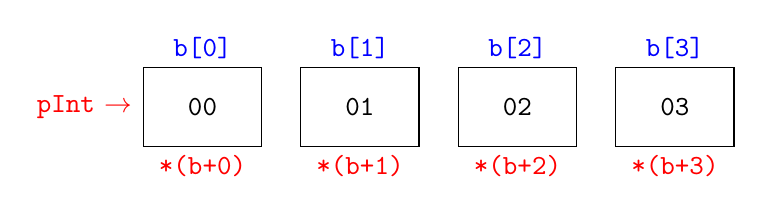
\begin{tikzpicture}
		\def\n{3} 	   % Number of plaintexts (rows)
		\def\xstart{0} % Start point for plaintexts on the x-axis
		\def\ystart{0} % Start point for plaintexts on the y-axis
		\def\xgap{2} % Horizontal gap between bytes
		\def\ygap{1.5} % Vertical gap between rows
		
		\def\bytesA{{"\texttt{00}", "\texttt{01}", "\texttt{02}", "\texttt{03}"}}
		
		\foreach \i/\rowbytes in {1/\bytesA} {
			\pgfmathsetmacro{\y}{\ystart - \i * \ygap}
			
			% Draw each byte in the row inside a box
			\foreach \j in {1, ..., 4} {
				\pgfmathsetmacro{\x}{\xstart + (\j-1) * \xgap}
				\ifnum\j=1
				\node[draw, rectangle, minimum width=1.5cm, minimum height=1cm] 
				at (\x, \y) {\pgfmathparse{\rowbytes[\j-1]}\pgfmathresult};
				\else
				\node[draw, rectangle, minimum width=1.5cm, minimum height=1cm] 
				at (\x, \y) {\pgfmathparse{\rowbytes[\j-1]}\pgfmathresult};
				\fi
			}
		}
		
		\node[red] at (-1.5,-1.5) {\texttt{pInt}\ $\to$\ };
		\node[red] at (0,-2.25) {\texttt{*(b+0)}};
		\node[red] at (2,-2.25) {\texttt{*(b+1)}};
		\node[red] at (4,-2.25) {\texttt{*(b+2)}};
		\node[red] at (6,-2.25) {\texttt{*(b+3)}};
		
		\node[blue] at (0,-.75) {\texttt{b[0]}};
		\node[blue] at (2,-.75) {\texttt{b[1]}};
		\node[blue] at (4,-.75) {\texttt{b[2]}};
		\node[blue] at (6,-.75) {\texttt{b[3]}};
	\end{tikzpicture}
\end{center}
\[\texttt{b}\iff\texttt{\&(b[0])}\iff\texttt{(u8*){\&}b[0]}\]
\lstinputlisting[style=C]{codes/little-endian/little-endian2.c}
\lstinputlisting[style=zsh]{codes/little-endian/little-endian-debug2}

\newpage
\[
\texttt{u8 b[4] = \{ 0x00, 0x01, 0x02, 0x03 \}};\implies\begin{cases}
	\texttt{u32 x = 0x03020100}; \\
	\texttt{u32 y = 0x00010203};
\end{cases}
\] \\
\lstinputlisting[style=C]{codes/little-endian/little-endian3.c}
\lstinputlisting[style=zsh]{codes/little-endian/little-endian-debug3}

\subsection{Marco}
\lstinputlisting[style=C]{codes/little-endian/little-endian4.c}
\lstinputlisting[style=zsh]{codes/little-endian/little-endian-debug4}

\newpage
\textbf{Byte to Word}
\begin{center}
	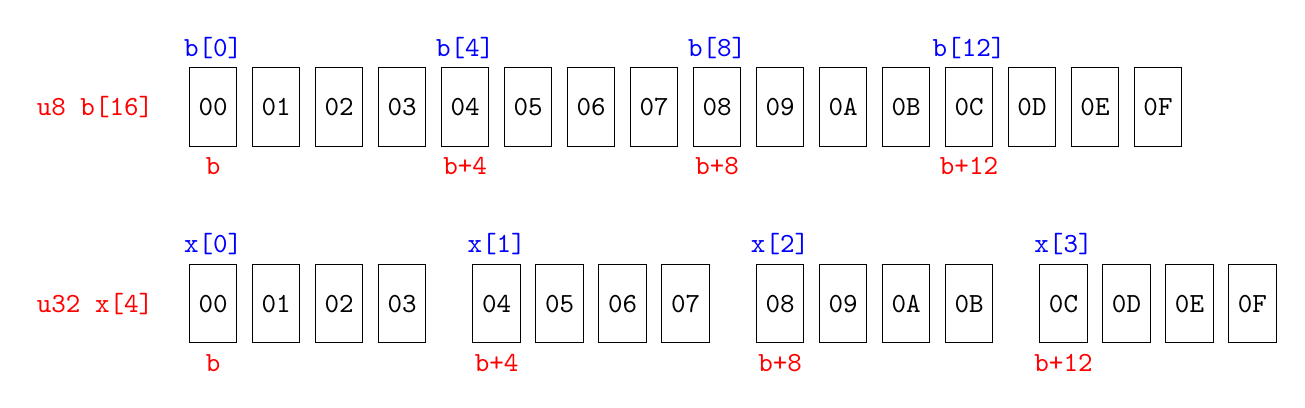
\begin{tikzpicture}
		\def\n{3} 	   % Number of plaintexts (rows)
		\def\xstart{0} % Start point for plaintexts on the x-axis
		\def\ystart{0} % Start point for plaintexts on the y-axis
		\def\xgap{.8} % Horizontal gap between bytes
		\def\ygap{1.5} % Vertical gap between rows
		
		\def\bytesA{{"\texttt{00}", "\texttt{01}", "\texttt{02}", "\texttt{03}",
					 "\texttt{04}", "\texttt{05}", "\texttt{06}", "\texttt{07}",
				 	 "\texttt{08}", "\texttt{09}", "\texttt{0A}", "\texttt{0B}",
			 	 	 "\texttt{0C}", "\texttt{0D}", "\texttt{0E}", "\texttt{0F}"}}
		
		\foreach \i/\rowbytes in {1/\bytesA} {
			\pgfmathsetmacro{\y}{\ystart - \i * \ygap}
			
			% Draw each byte in the row inside a box
			\foreach \j in {1, ..., 16} {
				\pgfmathsetmacro{\x}{\xstart + (\j-1) * \xgap}
				\ifnum\j=1
				\node[draw, rectangle, minimum width=.5cm, minimum height=1cm] 
				at (\x, \y) {\pgfmathparse{\rowbytes[\j-1]}\pgfmathresult};
				\else
				\node[draw, rectangle, minimum width=.5cm, minimum height=1cm] 
				at (\x, \y) {\pgfmathparse{\rowbytes[\j-1]}\pgfmathresult};
				\fi
			}
		}
		
		\node[red] at (-1.5,-1.5) {\texttt{u8 b[16]}};
		\node[red] at (0,-2.25) {\texttt{b}};
		\node[red] at (3.2,-2.25) {\texttt{b+4}};
		\node[red] at (6.4,-2.25) {\texttt{b+8}};
		\node[red] at (9.6,-2.25) {\texttt{b+12}};
		
		\node[blue] at (0,-.75) {\texttt{b[0]}};
		\node[blue] at (3.2,-.75) {\texttt{b[4]}};
		\node[blue] at (6.4,-.75) {\texttt{b[8]}};
		\node[blue] at (9.6,-.75) {\texttt{b[12]}};
		\begin{scope}[yshift=-2.5cm]
			\def\n{3} 	   % Number of plaintexts (rows)
			\def\xstart{0} % Start point for plaintexts on the x-axis
			\def\ystart{0} % Start point for plaintexts on the y-axis
			\def\xgap{.8} % Horizontal gap between bytes
			\def\ygap{1.5} % Vertical gap between rows
			
			\def\bytesA{{"\texttt{00}", "\texttt{01}", "\texttt{02}", "\texttt{03}"}}
			\def\bytesB{{"\texttt{04}", "\texttt{05}", "\texttt{06}", "\texttt{07}"}}
			\def\bytesC{{"\texttt{08}", "\texttt{09}", "\texttt{0A}", "\texttt{0B}"}}
			\def\bytesD{{"\texttt{0C}", "\texttt{0D}", "\texttt{0E}", "\texttt{0F}"}}	
			
			\foreach \i/\rowbytes in {0/\bytesA, 4.5/\bytesB, 9/\bytesC, 13.5/\bytesD} {
%				\pgfmathsetmacro{\y}{\ystart - \i * \ygap}
				
				% Draw each byte in the row inside a box
				\foreach \j in {1, ..., 4} {
					\pgfmathsetmacro{\x}{\xstart + (\j-1) * \xgap}
					\ifnum\j=1
					\node[draw, rectangle, minimum width=.5cm, minimum height=1cm] 
					at (\x + \i * \xgap, \ystart-1.5) {\pgfmathparse{\rowbytes[\j-1]}\pgfmathresult};
					\else
					\node[draw, rectangle, minimum width=.5cm, minimum height=1cm] 
					at (\x + \i * \xgap, \ystart-1.5) {\pgfmathparse{\rowbytes[\j-1]}\pgfmathresult};
					\fi
				}
			}
			
			\node[red] at (-1.5,-1.5) {\texttt{u32 x[4]}};
			\node[red] at (0,-2.25) {\texttt{b}};
			\node[red] at (3.6,-2.25) {\texttt{b+4}};
			\node[red] at (7.2,-2.25) {\texttt{b+8}};
			\node[red] at (10.8,-2.25) {\texttt{b+12}};
			
			\node[blue] at (0,-.75) {\texttt{x[0]}};
			\node[blue] at (3.6,-.75) {\texttt{x[1]}};
			\node[blue] at (7.2,-.75) {\texttt{x[2]}};
			\node[blue] at (10.8,-.75) {\texttt{x[3]}};
		\end{scope}
	\end{tikzpicture}
\end{center}

\lstinputlisting[style=C]{codes/little-endian/little-endian5.c}
\lstinputlisting[style=zsh]{codes/little-endian/little-endian-debug5}
\vspace{50pt}
\textbf{Word to Byte}
\begin{center}
	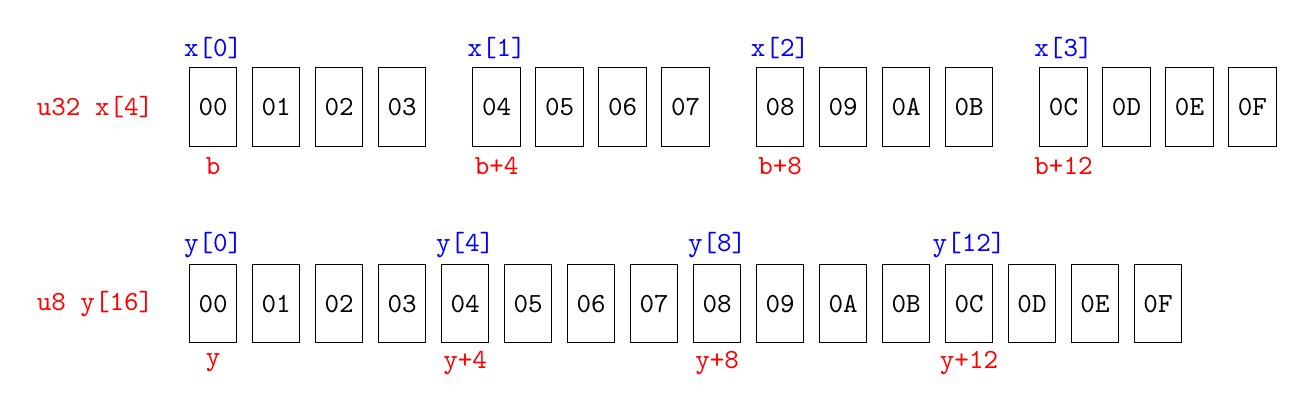
\begin{tikzpicture}
		\def\n{3} 	   % Number of plaintexts (rows)
		\def\xstart{0} % Start point for plaintexts on the x-axis
		\def\ystart{0} % Start point for plaintexts on the y-axis
		\def\xgap{.8} % Horizontal gap between bytes
		\def\ygap{1.5} % Vertical gap between rows
		
		\def\bytesA{{"\texttt{00}", "\texttt{01}", "\texttt{02}", "\texttt{03}",
				"\texttt{04}", "\texttt{05}", "\texttt{06}", "\texttt{07}",
				"\texttt{08}", "\texttt{09}", "\texttt{0A}", "\texttt{0B}",
				"\texttt{0C}", "\texttt{0D}", "\texttt{0E}", "\texttt{0F}"}}
		
		\foreach \i/\rowbytes in {1/\bytesA} {
			\pgfmathsetmacro{\y}{\ystart - \i * \ygap}
			
			% Draw each byte in the row inside a box
			\foreach \j in {1, ..., 16} {
				\pgfmathsetmacro{\x}{\xstart + (\j-1) * \xgap}
				\ifnum\j=1
				\node[draw, rectangle, minimum width=.5cm, minimum height=1cm] 
				at (\x, \y) {\pgfmathparse{\rowbytes[\j-1]}\pgfmathresult};
				\else
				\node[draw, rectangle, minimum width=.5cm, minimum height=1cm] 
				at (\x, \y) {\pgfmathparse{\rowbytes[\j-1]}\pgfmathresult};
				\fi
			}
		}
		
		\node[red] at (-1.5,-1.5) {\texttt{u8 y[16]}};
		\node[red] at (0,-2.25) {\texttt{y}};
		\node[red] at (3.2,-2.25) {\texttt{y+4}};
		\node[red] at (6.4,-2.25) {\texttt{y+8}};
		\node[red] at (9.6,-2.25) {\texttt{y+12}};
%		\node[red] at (12,-2.25) {\texttt{y+15}};
		
		\node[blue] at (0,-.75) {\texttt{y[0]}};
		\node[blue] at (3.2,-.75) {\texttt{y[4]}};
		\node[blue] at (6.4,-.75) {\texttt{y[8]}};
		\node[blue] at (9.6,-.75) {\texttt{y[12]}};
%		\node[blue] at (12,-.75) {\texttt{y[15]}};
		\begin{scope}[yshift=+2.5cm]
			\def\n{3} 	   % Number of plaintexts (rows)
			\def\xstart{0} % Start point for plaintexts on the x-axis
			\def\ystart{0} % Start point for plaintexts on the y-axis
			\def\xgap{.8} % Horizontal gap between bytes
			\def\ygap{1.5} % Vertical gap between rows
			
			\def\bytesA{{"\texttt{00}", "\texttt{01}", "\texttt{02}", "\texttt{03}"}}
			\def\bytesB{{"\texttt{04}", "\texttt{05}", "\texttt{06}", "\texttt{07}"}}
			\def\bytesC{{"\texttt{08}", "\texttt{09}", "\texttt{0A}", "\texttt{0B}"}}
			\def\bytesD{{"\texttt{0C}", "\texttt{0D}", "\texttt{0E}", "\texttt{0F}"}}	
			
			\foreach \i/\rowbytes in {0/\bytesA, 4.5/\bytesB, 9/\bytesC, 13.5/\bytesD} {
				%				\pgfmathsetmacro{\y}{\ystart - \i * \ygap}
				
				% Draw each byte in the row inside a box
				\foreach \j in {1, ..., 4} {
					\pgfmathsetmacro{\x}{\xstart + (\j-1) * \xgap}
					\ifnum\j=1
					\node[draw, rectangle, minimum width=.5cm, minimum height=1cm] 
					at (\x + \i * \xgap, \ystart-1.5) {\pgfmathparse{\rowbytes[\j-1]}\pgfmathresult};
					\else
					\node[draw, rectangle, minimum width=.5cm, minimum height=1cm] 
					at (\x + \i * \xgap, \ystart-1.5) {\pgfmathparse{\rowbytes[\j-1]}\pgfmathresult};
					\fi
				}
			}
			
			\node[red] at (-1.5,-1.5) {\texttt{u32 x[4]}};
			\node[red] at (0,-2.25) {\texttt{b}};
			\node[red] at (3.6,-2.25) {\texttt{b+4}};
			\node[red] at (7.2,-2.25) {\texttt{b+8}};
			\node[red] at (10.8,-2.25) {\texttt{b+12}};
			
			\node[blue] at (0,-.75) {\texttt{x[0]}};
			\node[blue] at (3.6,-.75) {\texttt{x[1]}};
			\node[blue] at (7.2,-.75) {\texttt{x[2]}};
			\node[blue] at (10.8,-.75) {\texttt{x[3]}};
		\end{scope}
	\end{tikzpicture}
\end{center}
\newpage
\lstinputlisting[style=C]{codes/little-endian/little-endian6.c}
\lstinputlisting[style=zsh]{codes/little-endian/little-endian-debug6}